% Diese Datei ist Teil des Buchs "Schreibe Dein Programm!"
% Das Buch ist lizensiert unter der Creative-Commons-Lizenz
% "Namensnennung - Weitergabe unter gleichen Bedingungen 4.0 International (CC BY-SA 4.0)"
% https://creativecommons.org/licenses/by-sa/4.0/deed.de

\chapter{Bäume}
\label{cha:trees}

\index{Baum}Bäume sind eine Form von Daten, die (wie Listen) besonders
oft in der Informatik vorkommt.  Oft ergeben sich baumförmige
Datendefinitionen aus der Problemstellung.  Wenn wir über diese
Datendefinitionen abstrahieren, entsteht eine universell verwendbare
Form von Daten, der \textit{Binärbaum}\index{Binärbaum}.  Diese
Binärbäume sind ähnlich vielseitig wie Listen und erlauben uns
außerdem, Daten so in Bäumen zu organisieren, dass wir sie schnell
wiederfinden können.

\section{Stammbäume}

Die Idee, den Baum als Metapher für eine bestimmte Form von Daten zu
benutzen, findet sich bereits in der Bibel, die Wörter wie
"<Baumstumpf"> und "<Spross"> benutzt, um Abstammmung zu beschreiben.
Erste bildliche Darstellungen von Stammbäumen sind aus diesen
Beschreibungen ab dem 11.\ Jahrhundert abgeleitet worden.

Das Stammbaum-Beispiel ist etwas ausgetreten, aber dennoch instruktiv.
In Stammbäumen sind in der Regel für eine Person ihr Name sowie
Verbindungen zu den beiden Eltern vermerkt.  Das führt zu folgender
Datendefinition.
%
\begin{lstlisting}
; Eine Person hat folgende Eigenschaften:
; - Name
; - Elternteil #1
; - Elternteil #2
\end{lstlisting}
%
Diese Definition lässt offen, um was für Daten es sich bei den beiden
Elternteilen handelt.  Natürlich sind es auch Personen, aber wenn wir
in einem Stammbaum weit genug nach oben gehen, sind diese irgendwann
unbekannt: Jeder konkrete Stammbaum endet irgendwo.  Wir brauchen also
auch noch eine Repräsentation für einen "<unbekannten Elternteil">
ohne (bekannte) Eigenschaften:
%
\begin{lstlisting}
; Ein unbekannter Elternteil hat keine Eigenschaften
(define-record unknown-parent
  make-unknown-parent
  unknown-parent?)
\end{lstlisting}
%
Daraus entsteht eine Datendefinition für "<Elternteil">:
%
\begin{lstlisting}
; Ein Elternteil ist eins der folgenden:
; - eine Person
; - ein unbekannter Elternteil
\end{lstlisting}
%
Diese~-- und die Datendefinition für "<Person"> können wir nun in Code
übersetzen:
%
\begin{lstlisting}
(define-record person
  make-person
  person?
  (person-name string)
  (person-parent-1 parent)
  (person-parent-2 parent))

(define parent
  (signature
   (mixed person unknown-parent)))
\end{lstlisting}
%
Für das unbekannte Elternteil stellen wir gleich mal einen Wert her:
%
\begin{lstlisting}
(define an-unknown-parent (make-unknown-parent))
\end{lstlisting}
%
Hier ein kleiner Stammbaum als Beispiel:
%
\begin{lstlisting}
(define slash
  (make-person "Slash"
               (make-person "Ola Hudson"
                            an-unknown-parent
                            an-unknown-parent)
               (make-person "Anthony Hudson"
                            an-unknown-parent
                            an-unknown-parent)))
(define london-hudson
  (make-person "London Hudson"
               slash
               (make-person "Perla Ferrar"
                            an-unknown-parent
                            an-unknown-parent)))
\end{lstlisting}
%
Wir schreiben nun eine Funktion, die feststellen soll, ob jemand der
Vorfahr einer Person ist, so etwa:
%
\begin{lstlisting}
; Ist jemand Vorfahr:in einer Person?
(: ancestor? (string person -> boolean))

(check-expect (ancestor? "Slash" london-hudson) #t)
(check-expect (ancestor? "Axl" london-hudson) #f)
\end{lstlisting}
%
Die Schablone für diese Funktion sieht folgendermaßen aus:
%
\begin{lstlisting}
(define ancestor?
  (lambda (name person)
    ...
    (person-name person)
    (person-parent-1 person)
    (person-parent-2 person)
    ...))
\end{lstlisting}
%
Was können wir mit diesen Bestandteilen anfangen?  Den Namen der
Person könnten wir mit dem gesuchten Namen vergleichen~-- wenn ja,
handelt es sich um einen Vorfahren:
%
\begin{lstlisting}
(define ancestor?
  (lambda (name person)
    (if (string=? name (person-name person))
        #t
        ...)
    (person-parent-1 person)
    (person-parent-2 person)
    ...))
\end{lstlisting}
%
Bei \lstinline{(person-parent-1 person)} und
\lstinline{(person-parent-2 person)} handelt es sich um gemischte
Daten.  Wir könnten die nötige Verzweigung direkt in
\lstinline{ancestor?} einbauen.  Genauso können wir eine separate
Funktion schreiben, welche die Frage beantwortet, ob ein Elternteil
Vorfahr ist.  Da es zwei Elternteile gibt, lohnt sich tendenziell eine
solche separate Funktion mit Kurzbeschreibung und Signatur wie folgt:
%
\begin{lstlisting}
; Ist jemand Vorfahr:in eines Elternteils?
(: parent-ancestor? (string parent -> boolean))
\end{lstlisting}
%
Diese Funktion schreiben wir gleich im Anschluss.  Aber ihre Signatur
ist genug, damit wir die Schablone in Funktion \lstinline{ancestor?}
weiter ausfüllen, indem wir überprüfen, ob Elternteil Nr.~1 oder Nr.~2
Vorfahr ist:
%
\begin{lstlisting}
(define ancestor?
  (lambda (name person)
    (if (string=? name (person-name person))
        #t
        (if (or (parent-ancestor? name (person-parent-1 person))
                (parent-ancestor? name (person-parent-2 person)))
            #t
            #f))))
\end{lstlisting}
%
Diese Funktion ist schon korrekt, aber sie könnte noch etwas eleganter
sein.  Der zweite \lstinline{if}-Ausdruck liefert \lstinline{#t}, falls
die Bedingung \lstinline{#t} und \lstinline{#f}, falls die Bedingung
\lstinline{#f} liefert: Es kommt also immer das Ergebnis der Bedingung
heraus.  Das ist eine allgemein anwendbare Regel:
%
\begin{lstlisting}
(if $b$ #t #f) $=$ $b$
\end{lstlisting}
%
Wir können \lstinline{ancestor?} also verkürzen auf:
%
\begin{lstlisting}
(define ancestor?
  (lambda (name person)
    (if (string=? name (person-name person))
        #t
        (or (parent-ancestor? name (person-parent-1 person))
            (parent-ancestor? name (person-parent-2 person))))))
\end{lstlisting}
%
Auch den verbleibenden \lstinline{if}-Ausdruck können wir noch
loswerden, weil er \lstinline{#t} ergibt, wenn die Bedingung
\lstinline{#t} ergibt oder wenn der \lstinline{or}-Ausdruck
\lstinline{#t} liefert.  Wir können deshalb die Funktion mit einem
großen \lstinline{or} schreiben:
%
\begin{lstlisting}
(define ancestor?
  (lambda (name person)
    (or (string=? name (person-name person))
        (parent-ancestor? name (person-parent-1 person))
        (parent-ancestor? name (person-parent-2 person)))))
\end{lstlisting}
%
Notwendig war diese Vereinfachung nicht, aber schöner sieht das
Resultat schon aus, finden wir!

Es fehlt noch die Hilfsfunktion \lstinline{parent-ancestor?}.  Hier
sind ein paar Tests:
%
\begin{lstlisting}
(check-expect (parent-ancestor? "Slash" london-hudson) #t)
(check-expect (parent-ancestor? "Axl" london-hudson) #f)
(check-expect (parent-ancestor? "Slash" an-unknown-parent) #f)
\end{lstlisting}
%
Gerüst und Schablone ergeben sich~-- wie immer~-- aus der
Datendefinition von \lstinline{parent}:
%
\begin{lstlisting}
(define parent-ancestor?
  (lambda (name parent)
    (cond
      ((person? parent) ...)
      ((unknown-parent? parent) ...))))
\end{lstlisting}
%
Für den ersten Fall können wir \lstinline{ancestor?} benutzen, im
zweiten Fall können wir mit \lstinline{#f} antworten:
%
\begin{lstlisting}
(define parent-ancestor?
  (lambda (name parent)
    (cond
      ((person? parent)
       (ancestor? name parent))
      ((unknown-parent? parent)
       #f))))
\end{lstlisting}
%
Fertig!

\begin{aufgabeinline}
  Ändere die Funktion \lstinline{ancestor?} dahingehend, dass eine
  Person nicht ihr eigener Vorfahr ist.
  Achte darauf, dass ansonsten die Funktion noch richtig arbeitet!
  Wird die Funktion einfacher?
\end{aufgabeinline}

\section{Binärbäume}
\label{sec:trees}

Wir schauen uns nochmal die Record-Defininiton von \lstinline{person}
an:
%
\begin{lstlisting}
(define-record person
  make-person
  person?
  (person-name string)
  (person-parent-1 parent)
  (person-parent-2 parent))
\end{lstlisting}
%
Vielleicht hat Dich das an eine Record-Definition aus
Kapitel~\ref{cha:selbstbezug} erinnert:
%
\begin{lstlisting}
(define-record confluence
  make-confluence
  confluence?
  (confluence-location  string)
  (confluence-main-stem river)
  (confluence-tributary river))
\end{lstlisting}
%
Die Struktur ist bei beiden Definitionen gleich.  Insbesondere
enthalten beide Definitionen jeweils zwei Selbstreferenzen.  Bei
\lstinline{person} ist die Selbstreferenz auf \lstinline{parent}, das
so definiert ist:
%
\begin{lstlisting}
(define parent
  (signature
   (mixed person unknown-parent)))
\end{lstlisting}
% 
Bei \lstinline{confluence} ist die Selbstreferenz auf
\lstinline{river}:
%
\begin{lstlisting}
(define river
  (signature (mixed creek confluence)))
\end{lstlisting}
%
Die jeweils anderen Fälle von \lstinline{parent} und
\lstinline{person} unterscheiden sich leicht:
%
\begin{lstlisting}
(define-record unknown-parent
  make-unknown-parent
  unknown-parent?)

(define-record creek
  make-creek
  creek?
  (creek-origin string))
\end{lstlisting}
%
In beiden steckt selbst aber keine Selbstreferenz mehr.  Beide
Datendefinitionen bilden baumartige Strukturen ab: Ein
\lstinline{person}- oder \lstinline{confluence}-Record bildet einen
Ast, der zweifach verzweigt.  Ein Baum endet jeweils bei
\lstinline{unknown-parent}- oder \lstinline{creek}-Records.  Weil die
"<inneren"> Äste immer zweifach verzweigen, handelt es sich in beiden
Fällen um \textit{Binärbäume}\index{Binärbaum}.  

Über diese beiden Sätze von Definitionen können wir abstrahieren.
Fangen wir mit \lstinline{person} und \lstinline{confluence} an.  Der
gängige Name für die Verzweigungen innerhalb eines Binärbaums ist
\textit{Knoten}\index{Knoten} oder \textit{innerer Knoten}, auf
Englisch \textit{node}.  Wir brauchen außerdem einen Namen für die
"<Namensdaten">, die bei beiden noch dabei sind.  Üblich ist
\textit{Markierung}\index{Markierung}, auf Englisch \textit{label}.
Die Signatur für den Selbstbezug nennen wir einfach \lstinline{tree}:
%
\begin{lstlisting}
(define-record node
  make-node node?
  (node-label string)
  (node-left-branch tree)
  (node-right-branch tree))
\end{lstlisting}
%
Das Wort "<branch"> heißt wörtlich übersetzt "<Zweig">, wir verwenden
aber die Begriffe "<linker Teilbaum"> und "<rechter Teilbaum">, was im
Deutschen üblicher ist.\index{Teilbaum}

Bei der Definition für \lstinline{tree} brauchen wir noch einen Namen
für die Werte an den Rändern des Baums~-- genannt
\textit{Blätter}\index{Blatt}, auf Englisch \textit{leaf}.
%
\begin{lstlisting}
(define tree
  (signature (mixed leaf node)))
\end{lstlisting}
%
Es fehlt noch die Definition von \lstinline{leaf}.  Hier ist es nicht
ganz so einfach, weil \lstinline{creek} noch einen Namen enthält,
\lstinline{unknown-parent} aber nicht.  Wir müssen also über beide
abstrahieren.  Einen Namen haben wir ja schon~-- \lstinline{leaf}~--
es fehlt noch das \lstinline{lambda}:
%
\begin{lstlisting}
(define tree-of
  (lambda (leaf)
    (signature (mixed leaf node))))
\end{lstlisting}
%
Das zieht noch eine weitere Änderung nach sich, weil \lstinline{tree}
ja in der Definition von \lstinline{node} verwendet wird.  Wir müssen
da entsprechend den \lstinline{leaf}-Parameter mit durchziehen:
%
\begin{lstlisting}
(define-record (node-of leaf)
  make-node node?
  (node-label string)
  (node-left-branch (tree-of leaf))
  (node-right-branch (tree-of leaf)))
\end{lstlisting}
%
Die Notation für die Abstraktion der Record-Signatur mit den
Extra-Klammern um \lstinline{(node-of leaf)} haben wir bisher erst
einmal gesehen, bei der Definition von \lstinline{cons-list-of} in
Abschnitt~\ref{function:cons-list-of} auf Seite~\pageref{function:cons-list-of}.

Wir könnten an dieser Stelle fertig sein.  Wir nehmen aber noch eine
Verallgemeinerung vor: Wie wir sehen werden, müssen die Markierungen
in Bäumen nicht unbedingt Zeichenketten sein~-- wir werden da noch
andere Arten von Werten ablegen wollen.  Darum abstrahieren wir auch
über die Signatur der Markierungen noch.  Außerdem reichen wir noch
die Datendefinitionen nach:
%
\begin{lstlisting}
; Ein Knoten besteht aus
; - Markierung
; - linken Ast
; - rechter Ast
(define-record (node-of leaf label)
  make-node node?
  (node-label label)
  (node-left-branch (tree-of leaf label))
  (node-right-branch (tree-of leaf label)))

; Ein Binärbaum ist entweder ein Blatt oder ein Knoten
(define tree-of
  (lambda (leaf label)
    (signature (mixed leaf (node-of leaf label)))))
\end{lstlisting}
%
Das nun ist die Definition eines Binärbaums in Reinform.  Hier sind
zwei Beispiele, bei denen wir einfach den Wert \lstinline{#f} als
Blatt verwendet haben:
%
\begin{lstlisting}
(: tree1 (tree-of false number))
(define tree1 (make-node 3 (make-node 4 #f (make-node 7 #f #f)) #f))
(: tree2 (tree-of false number))
(define tree2 (make-node 17 (make-node 3 #f tree1) #f))
\end{lstlisting}
%
Hier ist noch ein weiteres Beispiel, bei dem die Blätter Zahlen sind
und die Markierungen Zeichenketten
\begin{lstlisting}
(: tree3 (tree-of number string))
(define tree3 (make-node "Axl"
                         (make-node "Slash" 17 
                                            (make-node "Duff" 14 23))
                         12))
\end{lstlisting}
%

\begin{figure}[tb]
  \centering
  \begin{minipage}{0.3\textwidth}
\begin{center}
  \lstinline{tree1}\\[1ex]
  \begin{tikzpicture}[level/.style={sibling distance=20mm/#1, level distance=10mm}]
    \node (three){3}
    child {node (four) {4}
      child {node {$\bullet$}} 
      child {node (seven) {7}
        child {node {$\bullet$}}
        child {node {$\bullet$}}
      }
    }
   child {node {$\bullet$}};
 \end{tikzpicture}
\end{center}
\end{minipage}
\begin{minipage}{0.3\textwidth}
\begin{center}
  \lstinline{tree2}\\[1ex]
\begin{tikzpicture}[level/.style={sibling distance=20mm/#1, level distance=10mm}]
    \node (seventeen){17}
    child {node (three0) {3}
      child {node {$\bullet$}} 
      child {node (three){3}
        child {node (four) {4}
          child {node {$\bullet$}} 
          child {node (seven) {7}
            child {node {$\bullet$}}
            child {node {$\bullet$}}
          }
        }
      }
   }
   child {node {$\bullet$}};
 \end{tikzpicture}
\end{center}
\end{minipage}
\begin{minipage}{0.3\textwidth}
\begin{center}
  \lstinline{tree3}\\[1ex]
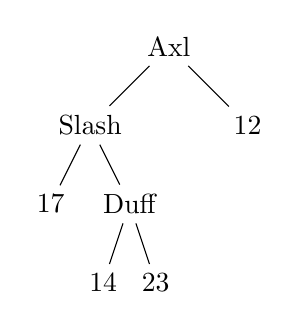
\begin{tikzpicture}[level/.style={sibling distance=20mm/#1, level distance=10mm}]
    \node (Axl){Axl}
    child {node (Slash) {Slash}
      child {node {17}} 
      child {node (Duff) {Duff}
        child {node {14}}
        child {node {23}}
      }
    }
   child {node {12}};
 \end{tikzpicture}
\end{center}
\end{minipage}
\caption{Beispielbäume}
  \label{fig:tree123}
\end{figure}

Abbildung~\ref{fig:tree123} stellt die drei Bäume \lstinline{tree1},
\lstinline{tree2} und \lstinline{tree3} grafisch dar.  Dort hat jeder
Baum erkennbar einen "<obersten"> Knoten, die sogenannte
\textit{Wurzel}\index{Wurzel}~-- ein Begriff, der im Zusammenhang mit
Bäumen häufig verwendet wird.  Bei dem Begriff muss immer mitgesagt
werden, \emph{wovon} die Wurzel gemeint ist. So ist 
\lstinline{tree1} ein Teil von \lstinline{tree2}.  Entsprechend steckt
die Wurzel von \lstinline{tree1} (der Knoten mit der 3) auch in
\lstinline{tree2} drin, aber die Wurzel von \lstinline{tree2} ist eben
der Knoten mit der 17.

Wir können \lstinline{tree-of} benutzen, um die Definition von
\lstinline{river} und \lstinline{parent} zu vereinfachen:
%
\begin{lstlisting}
(define river (tree-of creek string))
(define river? node?)
(define make-confluence make-node)
(define confluence-location node-label)
(define confluence-main-stem node-left-branch)
(define confluence-tributary node-right-branch)
\end{lstlisting}
%
\begin{aufgabeinline}
  Definiere \lstinline{person} mit Hilfe von \lstinline{tree-of}!
\end{aufgabeinline}
%
Auf Bäumen kann man alle möglichen Sachen berechnen.  Ein Beispiel ist
die \textit{Tiefe}\index{Tiefe!eines Baums}, also die maximale Anzahl
Knoten auf dem Weg zu einem Blatt.  (Manchmal heißt diese Größe auch
die \textit{Höhe}\index{Höhe!eines Baums} eines Baums.)  Für die Tiefe
des Baums sind die Signaturen der Blätter und Markierungen egal:
%
\begin{lstlisting}
; Tiefe eines Baums berechnen
(: depth ((tree-of %leaf %label) -> natural))
\end{lstlisting}
%
Hier sind zwei Testfälle:
%
\begin{lstlisting}
(check-expect (depth tree1) 3)
(check-expect (depth tree2) 5)
\end{lstlisting}
%
Bei \lstinline{tree1} sind es die Knoten mit den Markierunen 3, 4 und
7, die den maximal langen Weg zu einem Blatt bilden.  Bei
\lstinline{tree2} sind es 17, 3, 3, 4, 7.

Es geht wieder los mit der Konstruktionsanleitung.  Wir brauchen die
Schablone für gemischte Daten als Eingabe.  Da die Datendefinition für
Binärbäume zwei Fälle hat, brauchen wir ein \lstinline{cond} mit zwei
Zweigen.  Beim ersten können wir Bedingungen mit \lstinline{node?}
bilden.  Die Blätter haben kein festes Prädikat, aber das sind einfach
alle Bäume, die keine Knoten sind~-- wir können also statt einer
Bedingung \lstinline{else} schreiben:
%
\begin{lstlisting}
(define depth
  (lambda (tree)
    (cond
      ((node? tree) ...)
      (else ... 0))))
\end{lstlisting}
%
In den Knoten stecken zwei Selbstbezüge, wir brauchen also zwei
rekursive Aufrufe:
%
\begin{lstlisting}
(define depth
  (lambda (tree)
    (cond
      ((node? tree)
       ...
       (depth (node-left-branch tree))
       (depth (node-right-branch tree))
       ...)
      (else ...))))
\end{lstlisting}
%
Für die Tiefe zählt nur der Weg mit der maximalen Anzahl von Knoten.
Außerdem müssen wir den Knoten in \lstinline{tree} noch mitzählen.
Blätter zählen überhaupt nicht:
%
\begin{lstlisting}
(define depth
  (lambda (tree)
    (cond
      ((node? tree)
       (+ 1
          (max (depth (node-left-branch tree))
               (depth (node-right-branch tree)))))
      (else 0))))
\end{lstlisting}
%
Fertig!
%
\begin{aufgabeinline}
  Schreibe eine Funktion, die alle Knoten eines Baums zählt!
\end{aufgabeinline}
\begin{aufgabeinline}
  Schreibe eine Funktion, die für einen Baum eine Liste aller Blätter
  des Baums liefert!
\end{aufgabeinline}

\section{Bäume für's Suchen}
\label{sec:search-trees}

Viele Probleme bei der Programmierung sind "<Suchprobleme">: Einen
Namen, eine Telefonummer, eine Bestellnummer aus einer Liste
heraussuchen.  Darum geht es in diesem Abschnitt und wir fangen damit
an, dass wir das Wort "<Liste"> wörtlich nehmen und eine Funktion wie
folgt schreiben:
%
\begin{lstlisting}
; ist Wert Element einer Liste?
(: member? (%a (list-of %a) -> boolean))
\end{lstlisting}
%
Wir haben eine Signaturvariable verwendet, weil es sich bei den
Listenelementen mal um Zahlen, mal um Zeichenketten, mal um etwas
anderes handeln kann.  Hier sind ein paar Testfälle:
%
\begin{lstlisting}
(check-expect (member? 5 empty) #f)
(check-expect (member? 2 (list 1 2 3)) #t)
(check-expect (member? "Slash" (list "Axl" "Slash")) #t)
(check-expect (member? "Buckethead" (list "Axl" "Slash")) #f)
\end{lstlisting}
%
Hier Gerüst und Schablone für Funktionen auf Listen:
%
\begin{lstlisting}
(define member?
  (lambda (element list)
    (cond
      ((empty? list) ...)
      ((cons? list)
       ... 
       (first list)
       (member? element (rest list))
       ...))))
\end{lstlisting}
%
Bei der leeren Liste kann die Funktion nur \lstinline{#f}
zurückgeben.  Bei der Cons-Liste legt die Schablone nahe, dass die
Funktion erst einmal prüfen sollte, ob \lstinline{(first list)} das
gesucht Element ist.

Klingt einfach, oder?  Aber \emph{wie} prüfen wir das?  Wir könnten
das hier hinschreiben:
%
\begin{lstlisting}
(= element (first list))
\end{lstlisting}
%
\ldots~aber das würde die Funktion auf Zahlen beschränken, weil
\lstinline{=} nur auf Zahlen funktioniert.  Für die beiden Testfälle
mit Zeichenketten müssten wir \lstinline{string=?} verwenden.  Wir
müssen also \lstinline{member?} über \lstinline{=} respektive
\lstinline{string=?} abstrahieren, noch bevor die Funktion überhaupt
fertig ist.  Wir brauchen wie immer einen weiteren Parameter und
nennen ihn \lstinline{equals?}:
%
\begin{lstlisting}
(define member?
  (lambda (equals? element list)
    (cond
      ((empty? list) ...)
      ((cons? list)
       ... 
       (first list)
       (member? equals? element (rest list))
       ...))))
\end{lstlisting}
%
(Aufpassen: Der rekursive Aufruf muss~-- wie immer~-- auch durch den
neuen Parameter erweitert werden.)

Jetzt können wir den Vergleich mit Hilfe von \lstinline{equals?}
durchführen und diesen mit einer binären Verzweigung verarbeiten:
%
\begin{lstlisting}
(define member?
  (lambda (equals? element list)
    (cond
      ((empty? list) #f)
      ((cons? list)
       (if (equals? element (first list))
           #t
           (member? equals? element (rest list)))))))
\end{lstlisting}
%
Signatur und Testfälle haben von dem neuen Parameter noch nichts
mitbekommen.  Die \lstinline{equals?}-Funktion akzeptiert zwei
Listenelemente und liefert ein boolesches Ergebnis.  Da die
Listenelemente die Signatur \lstinline{%a}
haben, sieht die Signaturdeklaration für \lstinline{member?} so aus:
%
\begin{lstlisting}
(: member? ((%a %a -> boolean) %a (list-of %a) -> boolean))
\end{lstlisting}
%
Bei den Testfällen müssen wir jeweils noch die richtige
Vergleichsfunktion übergeben.  Das ist \lstinline{=} für Zahlen und
\lstinline{equals?} für Zeichenketten.
%
\begin{lstlisting}
(check-expect (member? = 5 empty) #f)
(check-expect (member? = 2 (list 1 2 3)) #t)
(check-expect (member? string=? "Slash" (list "Axl" "Slash")) #t)
(check-expect (member? string=? "Buckethead" (list "Axl" "Slash")) #f)
\end{lstlisting}
%
Fertig!

Allerdings hat \lstinline{member?} einen Nachteil: Bei kurzen Listen
oder wenn das gesuchte Element am Anfang der Liste steht, wird
\lstinline{member?} ziemlich schnell fertig.  Aber stell Dir vor, die
Liste hat ein paar Millionen Elemente und das gesuchte Element ist am
Ende.  Oder gar nicht drin: Dann muss \lstinline{member?} die gesamte
Liste abklappern.
%
\begin{aufgabeinline}
  Schreibe mit Hilfe von \lstinline{member?} eine Funktion, die von
  zwei Listen alle Elemente liefert, die in beiden Listen stehen, also
  deren Schnittmenge.  Wie lange braucht diese Funktion im
  ungünstigsten Fall?
\end{aufgabeinline}
%
Kann irgendwie schneller herausfinden, ob ein Wert Element einer Menge
ist oder nicht?  In der Tat ist das möglich, aber nicht mit Listen:
Wir brauchen eine andere Struktur, um das Suchen zu beschleunigen~--
Bäume.

\begin{figure}[tb]
\begin{tikzpicture}[level/.style={sibling distance=60mm/#1}]
\node (z){$M$}
  child {node (a) {$B$}
    child {node (b) {$A$}
      child {node {$\bullet$}} 
      child {node {$\bullet$}}
    }
    child {node (g) {$D$}
      child {node {$\bullet$}}
      child {node {$\bullet$}}
    }
  }
  child {node (j) {$O$}
    child {node (k) {$N$}
      child {node {$\bullet$}}
      child {node {$\bullet$}}
    }
    child {node (l) {$R$}
      child {node {$\bullet$}}
      child {node {$\bullet$}}
    }
  };
\end{tikzpicture}
  \caption{Sortierter Baum über Buchstaben}
  \label{fig:searchtree}
\end{figure}

Schau Dir mal Abbildung~\ref{fig:searchtree} an.  In diesem Baum musst
Du nicht alle Elemente anschauen, um ein bestimmtes Element zu
finden.  Das liegt daran, dass die Buchstaben in dem Baum auf
bestimmte Art nach dem Alphabet sortiert sind:

Die Wurzel mit der Markierung $M$ hat zwei Teilbäume~-- die
Markierungen des linken Teilbaums liegen allesamt \emph{vor} $M$ im
Alphabet, alle Markierungen des rechten Teilbaums \emph{nach} $M$.
Wenn Du also nach einem Buchstaben suchst~-- nehmen wir mal $D$~--
dann weißt Du, wenn Du die Wurzel mit $M$ siehst, dass $D$ im linken
Teilbaum von $M$~-- mit der Markierung $B$ und von da aus im rechten
Teilbaum von $B$ stehen muss.  Die Knoten $A$, $O$, $N$, $R$ kannst Du
ignorieren.

Die Suche braucht also höchstens so viele Schritte wie der Baum tief
ist.  Das ist schonmal besser, als in der Liste zu suchen, wo wir
potenziell alle Elemente anschauen müssen.

Programmieren wir das also!

Wir fangen mit einem sortierten Baum über reellen Zahlen an.
(Reelle Zahlen deshalb, weil wir sie einfach mit \lstinline{=} und
\lstinline{<} vergleichen können.  Wir verallgemeinern das später.)
Die Zahlen kleben als Markierungen an den Knoten.  An den Blättern
steht nichts relevantes, wir benutzen deshalb immer \lstinline{#f}.
Entsprechend sehen Kurzbeschreibung und Signatur so aus:
%
\begin{lstlisting}
; Ist eine Zahl in einem sortierten Baum vorhanden? 
(: tree-member? (real (tree-of false real) -> boolean))
\end{lstlisting}
%
Die Signatur \lstinline{false}\index{false@\texttt{false}} ist neu:
Sie beschreibt nur den Wert \lstinline{#f}.  Entsprechend gibt es
natürlich auch eine Signatur
\lstinline{true}\index{true@\texttt{true}} für \lstinline{#t}.

Als Beispielbaum für die Tests benutzen wir diesen hier:
%
\begin{lstlisting}
(define tree4
   (make-node 5
              (make-node 3 #f #f)
              (make-node 17
                         (make-node 10 #f (make-node 12 #f #f))
                         #f)))
\end{lstlisting}
%
Hier sind ein paar Tests:
%
\begin{lstlisting}
(check-expect (tree-member? 5 tree4) #t)
(check-expect (tree-member? 17 tree4) #t)
(check-expect (tree-member? 3 tree4) #t)
(check-expect (tree-member? 10 tree4) #t)
(check-expect (tree-member? 2 tree4) #f)
\end{lstlisting}
%
Hier ist das Gerüst:
\begin{lstlisting}
(define tree-member?
  (lambda (value tree)
    ...))
\end{lstlisting}
%
In die Schablone für Bäume tragen wir gleich den zweiten Fall ein:
Wenn die Funktion ein Blatt erreicht, dann ist das \lstinline{value}
definitiv nicht im Baum, das Ergebnis dann \lstinline{#f}:
%
\begin{lstlisting}
(define tree-member?
  (lambda (value tree)
    (cond
      ((node? tree)
       ...
       (node-label tree)
       (tree-member? value (node-left-branch tree))
       (tree-member? value (node-right-branch tree))
       ...
      (else #f)))))
\end{lstlisting}
%
Bei Knoten können wir drei Fälle unterscheiden: Wenn die Markierung
gerade das gesucht \lstinline{value} ist, wenn \lstinline{value}
kleiner ist als die Markierung (also im linken Teilbaum stehen muss)
und wenn sie größer ist.  Daraus ergibt sich folgende
Weiterentwicklung:
\begin{lstlisting}
(define tree-member?
  (lambda (value tree)
    (cond
      ((node? tree)
      ...
      (tree-member? value (node-left-branch tree)))
      (tree-member? value (node-right-branch tree))
      ...
      (cond
         ((= value (node-label tree)) #t)
         ((< value (node-label tree)) ...
         (else ...)))
      (else #f))))
\end{lstlisting}
%
Da \lstinline{(node-label tree)} zweimal vorkommt, machen wir dafür
eien Definition und setzen die Bestandteile der Schablone so zusammen:
%
\begin{lstlisting}
(define tree-member?
  (lambda (value tree)
    (cond
      ((node? tree)
       (define label (node-label tree))
       (cond
         ((= value label) #t)
         ((< value label)
          (tree-member? value (node-left-branch tree)))
         (else
          (tree-member? value (node-right-branch tree)))))
      (else #f))))
\end{lstlisting}
%
Fertig!

\section{Sortierte Bäume herstellen}

In den Testfällen für \lstinline{tree-member?} haben wir immer den
Baum \lstinline{tree4} vwerwendet, den wir direkt mit
\lstinline{make-node} konstruiert haben.  Dabei mussten wir selbst
darauf achten, dass er auch sortiert ist.  In diesem Abschnitt
automatisieren wir diese Konstruktion, dann kann dabei auch kein
Fehler passieren.  (Wenn wir korrekt programmieren zumindest.)

Wir schreiben dafür eine Funktion, die ein neues Element in einen
bestehenden sortierten Baum einfügt.  Kurzbeschreibung und Signatur
sind wie folgt:
%
\begin{lstlisting}
; Zahl in sortierten Baum einfügen 
(: tree-insert (real (tree-of false real) -> (tree-of false real)))
\end{lstlisting}
%
Testfälle brauchen wir als nächstes.  Wir könnten das so machen wie
immer: Wir schreiben einen Aufruf von \lstinline{tree-member?} hin und
den Ergebniswert, den wir uns erhoffen.  In diesem Fall aber ist es
gar nicht so wichtig, was der Ergebniswert genau ist.  Wichtig ist,
dass ein eingefügtes Element im Ergebnisbaum auch drin ist.  Außerdem
ist es mühsam, immer den ganzen Baum hinzuschreiben.  Darum benutzen
wir \lstinline{tree-member?}, um \lstinline{tree-insert} zu testen.
%
\begin{lstlisting}
(check-expect (tree-member? 5 (tree-insert 5 tree4)) #t)
(check-expect (tree-member? 11 (tree-insert 11 tree4)) #t)
\end{lstlisting}
%
Später werden wir feststellen, dass \lstinline{tree-insert}
unterschiedliche sortierte Bäume liefern kann, die allesamt korrekt
sind.
%
\begin{aufgabeinline}
  Die beiden Tests erwarten jeweils, dass \lstinline{#t} bei
  \lstinline{tree-member?} herauskommt.  Wäre es sinnvoll, auch noch
  welche mit \lstinline{#f} zu schreiben?
\end{aufgabeinline}
%
Wenn Du ein mulmiges Gefühl bei den spärlichen beiden Tests hast:
richtig!  In Kapitel~\ref{cha:properties} auf
Seite~\pageref{cha:properties} werden wir zeigen, wie man Funktionen
wie \lstinline{tree-insert} besser testet.

Aber jetzt geht's erst einmal mit der Funktion selbst los.  Gerüst und
Schablone sind genau wie bei \lstinline{tree-member?}:
%
\begin{lstlisting}
(define tree-insert
  (lambda (value tree)
    (cond
      ((node? tree)
        ...
        (tree-insert value (node-left-branch tree))
        (tree-insert value (node-right-branch tree))
        ...)
      (else ...))))
\end{lstlisting}
%
Die Fallunterscheidung bei Knoten ist ebenfalls wie in
\lstinline{tree-member?}, darum können wir auch die Verzweigung aus
der dortigen Schablone übernehmen:
%
\begin{lstlisting}
(define tree-insert
  (lambda (value tree)
    (cond
      ((node? tree)
        ...
        (tree-insert value (node-left-branch tree))
        (tree-insert value (node-right-branch tree))
        ...
        (cond
         ((= value (node-label tree)) ...)
         ((< value (node-label tree)) ...)
         (else ...)))
      (else ...))))
\end{lstlisting}
%
Auch hier ist der erste Fal einfach: Wenn \lstinline{value} gerade die
Markierung eines Knotens ist, dann enthält der Baum den Wert bereits,
die Funktion muss nichts einfügen und kann einfach \lstinline{tree}
liefern.  Auch für den Fall, dass \lstinline{tree} ein Blatt ist (das
letzte \lstinline{else}), ist es recht einfach: Wir konstruieren einen
neuen, einelementigen Baum:
%
\begin{lstlisting}
(define tree-insert
  (lambda (value tree)
    (cond
      ((node? tree)
        ...
        (tree-insert value (node-left-branch tree))
        (tree-insert value (node-right-branch tree))
        ...
        (cond
         ((= value (node-label tree)) tree)
         ((< value (node-label tree)) ...)
         (else ...)))
      (else (make-node value #f #f)))))
\end{lstlisting}
%
Es bleiben noch zwei Fälle, in denen der einzufügende Wert links
beziehungsweise rechts von der Knotenmarkierung liegt.  Er muss
entsprechend im linken oder rechten Teilbaum eingefügt werden: Genau
das erledigen die beiden rekursiven Aufrufe aus der Schablone.  Der
jeweils andere Teilbaum bleibt so wie er ist:
%
\begin{lstlisting}
(define tree-insert
  (lambda (value tree)
    (cond
      ((node? tree)
       (cond
         ((= value (node-label tree)) tree)
         ((< value (node-label tree))
          (make-node (node-label tree)
                     (tree-insert value (node-left-branch tree))
                     (node-right-branch tree)))
         (else
          (make-node (node-label tree)
                     (node-left-branch tree)
                     (tree-insert value (node-right-branch tree))))))
      (else
       (make-node value #f #f)))))
\end{lstlisting}
%
Fertig!

\section{Suchbäume}

Unsere Funktionen \lstinline{tree-member?} und \lstinline{tree-insert}
funktionieren nur auf Zahlen. Die Bäume aus den
Abbildungen~\ref{fig:searchtree} und \ref{fig:degenerated-searchtree}
enthalten aber beide Buchstaben.  Wenn wir andere Werte als Zahlen
zulassen wollen, müssen wir wieder einmal abstrahieren über alles, was
mit Zahlen zu tun hat.

Schau Dir nochmal die Definition von \lstinline{tree-member?} an: Es
gibt zwei Stellen, die "<zahlenspezifisch"> sind, nämlich
\lstinline{=} und \lstinline{<}.  Wenn Zeichenketten in einem
sortierten Baum unterbringen wollten, müssten wir da
\lstinline{string=?} und \lstinline{string<?} hinschreiben.

\begin{aufgabeinline}
  Abstrahiere \lstinline{tree-member?} und \lstinline{tree-insert}
  über \lstinline{=} und \lstinline{<}.

  Übergib mal statt \lstinline{<} die Funktion \lstinline{>}.
  Funktionieren \lstinline{tree-member?} und \lstinline{tree-insert}
  dann noch korrekt?  Wie unterscheiden sich die Bäume, die mit
  \lstinline{<} aus \lstinline{tree-insert} herauskommen von denen mit
  \lstinline{>}?
\end{aufgabeinline}

Die abstrahierten Versionen von \lstinline{tree-member?} und
\lstinline{tree-insert} haben einen Nachteil: Bei jedem Aufruf dieser
Funktionen müssen wir die beiden Argumente für \lstinline{=} und
\lstinline{<} hinschreiben.  Das nervt und ist jedesmal eine
Gelegenheit für einen Fehler, weil wir das vollkommen konsistent
machen müssen.

Wir wollen also versuchen, ohne diese zusätzlichen Parameter
auszukommen.  Dazu benutzen wir einen Trick und packen die Funktionen
für \lstinline{=} und \lstinline{<} zusammen mit \lstinline{tree}.
Das Ergebnis heißt \textit{Suchbaum}\index{Suchbaum}.  Heraus kommt
folgende Datendefinition:
%
\begin{lstlisting}
; Ein Suchbaum besteht aus
; - Funktion für =
; - Funktion für <
; - Binärbaum
\end{lstlisting}
%
Um die Definition in Code umzusetzen, benutzen wir eine
Record-Definition.  Diesmal abstrahieren wir über die Signatur der
Elemente mit einem Signatur-Parameter namens \lstinline{element}:
%
\begin{lstlisting}
(define-record (search-tree-of element)
  make-search-tree search-tree?
  (search-tree-label-=?-function (element element -> boolean))
  (search-tree-label-<?-function (element element -> boolean))
  (search-tree-tree (tree-of false element)))
\end{lstlisting}
%
Vergleiche die Signatur von \lstinline{search-tree-tree} mit der
Signatur der Bäume bei \lstinline{tree-member?} und
\lstinline{tree-insert}!

Hier ist der Suchbaum aus Abbildung~\ref{fig:searchtree} auf
Seite~\pageref{fig:searchtree}:
%
\begin{lstlisting}
(define search-tree1
  (make-search-tree
   string=? string<?
   (make-node "M"
              (make-node "B"
                         (make-node "A" #f #f)
                         (make-node "D" #f #f))
              (make-node "O"
                         (make-node "N" #f #f)
                         (make-node "R" #f #f)))))
\end{lstlisting}
%
Wir schreiben nun eine Variante von \lstinline{tree-member?},
die Suchbäume statt "<normale"> Bäume
akzeptieren.  Hier Kurzbeschreibung, Signatur und Tests für die
Funktion für das Suchen:
%
\begin{lstlisting}
; festellen, ob Element in Suchbaum vorhanden ist
(: search-tree-member? (%a (search-tree-of %a) -> boolean))
(check-expect (search-tree-member? "M" search-tree1) #t)
(check-expect (search-tree-member? "D" search-tree1) #t)
(check-expect (search-tree-member? "N" search-tree1) #t)
(check-expect (search-tree-member? "R" search-tree1) #t)
(check-expect (search-tree-member? "Z" search-tree1) #f)
\end{lstlisting}
%
Hier ist das Gerüst für die Funktionsdefinition, zusammen mit der
Schablone für \lstinline{search-tree}:
%
\begin{lstlisting}
(define search-tree-member?
  (lambda (value search-tree)
    ...
    (search-tree-label-=?-function search-tree)
    (search-tree-label-<?-function search-tree)
    (search-tree-tree search-tree)
    ...))
\end{lstlisting}
%
Jetzt könnten wir natürlich alles wie immer ausprogrammieren.  Viel
einfacher aber ist es, wenn wir die existierende Funktion
\lstinline{tree-member?} wiederverwenden: Wir haben ja genau das
gleiche vor, was die Funktion schon macht.  Dazu kopieren wir sie
einfach in den Rumpf:
%
\begin{lstlisting}
(define search-tree-member?
  (lambda (value search-tree)
    ...
    (search-tree-label-=?-function search-tree)
    (search-tree-label-<?-function search-tree)
    (search-tree-tree search-tree)
    (define tree-member?
      (lambda (value tree)
        (cond
          ((node? tree)
           (define label (node-label tree))
           (cond
             ((= value label) #t)
             ((< value label)
              (tree-member? value (node-left-branch tree)))
             (else
              (tree-member? value (node-right-branch tree)))))
          (else #f))))
    ...))
\end{lstlisting}
%
Wir müssen allerdings noch über \lstinline{=} und \lstinline{<}
abstrahieren.  Dazu denken wir uns erstmal nur neue Namen aus, nämlich
\lstinline{label=?} für \lstinline{=} und \lstinline{label<?} für \lstinline{<}:
%
\begin{lstlisting}
(define search-tree-member?
  (lambda (value search-tree)
    ...
    (search-tree-label-=?-function search-tree)
    (search-tree-label-<?-function search-tree)
    (search-tree-tree search-tree)
    (define tree-member?
      (lambda (value tree)
        (cond
          ((node? tree)
           (define label (node-label tree))
           (cond
             ((label=? value label) #t)
             ((label<? value label)
              (tree-member? value (node-left-branch tree)))
             (else
              (tree-member? value (node-right-branch tree)))))
          (else #f))))
    ...))
\end{lstlisting}
%
Anders als sonst legen wir aber keine Parameter für
\lstinline{label=?} und \lstinline{label<?} an: Die Funktionen
dafür stehen ja schon in der Schablone, wir müssen ihnen nur die
richtigen Namen geben mit Hilfe von lokalen Definitionen:
%
\begin{lstlisting}
(define search-tree-member?
  (lambda (value search-tree)
    (define label=? (search-tree-label-=?-function search-tree))
    (define label<? (search-tree-label-<?-function search-tree))
    ...
    (search-tree-tree search-tree)
    ...
    (define tree-member? ...)
    ...)))
\end{lstlisting}
%
Zu guter letzt brauchen wir noch einen Aufruf von \lstinline{tree-member?}
im Rumpf von \lstinline{search-tree-member?}, damit es auch losgeht.
Dafür verbrauchen wir den letzten Baustein aus der Schablone:
%
\begin{lstlisting}
(define search-tree-member?
  (lambda (value search-tree)
    (define label=? (search-tree-label-=?-function search-tree))
    (define label<? (search-tree-label-<?-function search-tree))
    (define tree-member?
      (lambda (value tree)
        (cond
          ((node? tree)
           (define label (node-label tree))
           (cond
             ((label=? value label) #t)
             ((label<? value label)
              (tree-member? value (node-left-branch tree)))
             (else
              (tree-member? value (node-right-branch tree)))))
          (else #f))))
    (tree-member? value (search-tree-tree search-tree))))
\end{lstlisting}
%
Fertig!

\begin{aufgabeinline}
  Schreibe entsprechend zu \lstinline{search-tree-member?} eine
  Funktion \lstinline{search-tree-insert} auf Basis von
  \lstinline{tree-insert}!
\end{aufgabeinline}

% FIXME: Aufgabe Baum -> Liste

\section{Sortierte Bäume sind effizienter als Listen}
  
Intuitiv ist die Idee mit dem sortierten Baum beim Suchen
effizienter.  Aber hält diese Intuition auch einer mathematischen
Untersuchung stand?  Betrachte dazu den Baum in "<Ebenen"> --
erste Ebene ist die Wurzel, die zweite Ebene deren Teilbäume, die
dritte Ebene wiederum deren Teilbäume undsoweiter.  Dann passen in
jede Ebene doppelt soviele Knoten wie in die Ebene darüber.

In einen Baum der Tiefe 1 passt auch nur $1 = 2^0$ Knoten, in einen
der Tiefe 2 passen $2^0 + 2^1 = 1+2 = 3$ Knoten, dann 7, dann 15
undsoweiter.  Dir fällt vielleicht auf, dass die Zahlen 1, 3, 7, 15
allesamt Vorgänger einer Zweierpotenz sind.  Wir können deshalb
versuchen, das zu einer Formel zu verallgemeinern.  Die Tiefe des
Baums heißt dabei $t$.  Dann nehmen wir an (oder hoffen zumindest),
dass für für alle 
%
\begin{displaymath}
  2^0 + ... + 2^{t-1} = \sum_{i=0}^{i=t-1} 2^i  = 2^t-1
\end{displaymath}
%
Da es sich bei $t$ um eine natürliche Zahl handelt, können wir
vollständige Induktion anwenden nach der Anleitung in
Abschnitt~\ref{sec:nat-induction-ka} auf
Seite~\pageref{sec:nat-induction-ka}.

Wir müssen also beweisen, dass für alle $t\in\mathbb{N}$ gilt:
%
\begin{displaymath}
  \sum_{i=0}^{i=t-1} 2^i  = 2^t-1
\end{displaymath}
%
$t=0$:
%
\begin{displaymath}
  \sum_{i=0}^{i=0-1} 2^i = 2^0 - 1
\end{displaymath}
%
Beweis:
%
\begin{eqnarray*}
  \sum_{i=0}^{i=-1} 2^i
  &=& 0\\
  &=& 1-1\\
  &=& 2^0 - 1
\end{eqnarray*}
%
(Vielleicht kommt Dir komisch vor, dass die Summe von $0$ bis $-1$
läuft.  Da es keine Zahl zwischen $0$ bis $-1$ gibt, ist die Summe
leer und deshalb das neutrale Element bezüglich der Addition.)

\smallskip

\noindent Induktionsvoraussetzung:
\begin{displaymath}
  \sum_{i=0}^{i=t-1} 2^i  = 2^t-1
\end{displaymath}
%
Induktionsschluss (zu zeigen):
%
\begin{displaymath}
    \sum_{i=0}^{i=(t+1)-1} 2^t = 2^{t+1} - 1
\end{displaymath}
%
Beweis:
%
\begin{eqnarray*}
  \sum_{i=0}^{i=(t+1)-1} 2^i
  &=& \sum_{i=0}^{i=t} 2^i\\
  &=& \sum_{i=0}^{i=t-1} 2^i + 2^t\\
  &=& 2^t-1 + 2^t \quad\textrm{Induktionsvoraussetzung}\\
  &=& 2^t\cdot 2 - 1\\
  &=& 2^{t+1} - 1
\end{eqnarray*}
%
Wozu ist diese Formel gut, fragst Du Dich vielleicht.  Nun, die rechte
Seite können wir umdrehen.  (Bei der linken Seite ist das
schwieriger.) Wenn die Anzahl der Knoten $k$ ist, dann gilt:
%
\begin{displaymath}
  \begin{array}{lrcl}
    & k &=& 2^t - 1\\
    \Longleftrightarrow & k + 1 &=& 2^t\\
    \Longleftrightarrow & \log_2(k+1) &=& t
  \end{array}
\end{displaymath}
%
Die $\log_2$ ist der sogenannte
\textit{Logarithmus}\index{Logarithmus} zur Basis 2, auch genannte
\textit{Zweierlogarithmus}\index{Zweierlogarithmus}.  Das ist die
Umkehrfunktion zur Exponentialfunktion mit der Basis 2.

\begin{figure}[tb]
  \centering
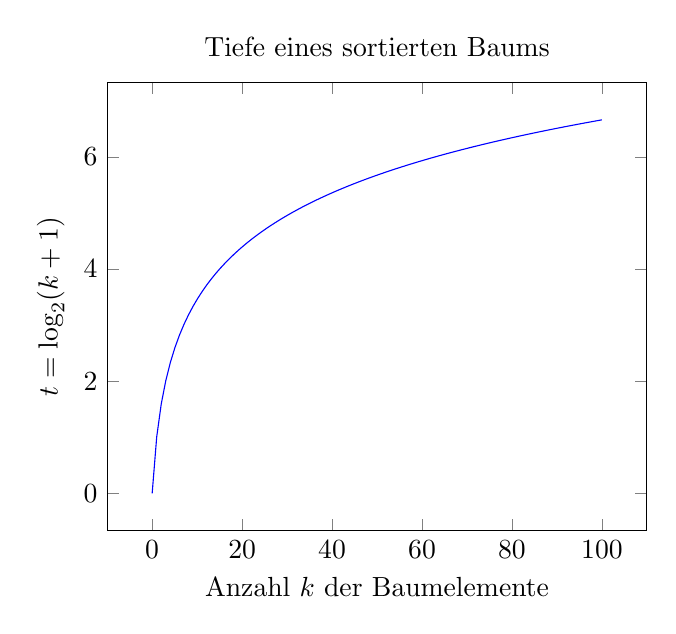
\begin{tikzpicture}
  \begin{axis}[
    title={Tiefe eines sortierten Baums },
    xlabel={Anzahl $k$ der Baumelemente},
    ylabel={$t = \log_2(k+1)$}
    ]
    \addplot [
    blue,
    domain=0:100,
    samples=100,
    ]
    {log2(x+1)}; 
  \end{axis}
\end{tikzpicture}
  \caption{Beziehung zwischen Anzahl von Knoten und Tiefe eines Binärbaums}
  \label{fig:log2}
\end{figure}

Schau Dir Abbildung~\ref{fig:log2} an: Da siehst Du, dass die Tiefe~--
mithin der Logarithmus~-- viel langsamer wächst als die Anzahl der
Knoten, und die Kurve immer flacher wird.  Diese Kurve erklärt, warum
das mit dem sortierten Baum eine gute Idee ist: Die Tiefe des Baums ist ja
die Anzahl der Elemente des Baums, die man abklappern muss, um das
gewünschte Element zu finden.  (Beziehungsweise herauszubekommen, dass
es nicht im Suchbaum ist.)  Das gilt allerdings nur, wenn der Suchbaum
"<voll besetzt"> ist.  Wir müssen uns also irgendwann Gedanken machen,
wie wir dafür sorgen, dass Suchbäume immer möglichst voll besetzt
sind.  Dazu kommen wir später.

\section{Suchbäume balancieren}

\begin{figure}[tb]
\begin{tikzpicture}[level/.style={sibling distance=60mm/#1}]
\node (z){$A$}
    child {node {$\bullet$}}
    child {node (b) {$B$}
      child {node {$\bullet$}}
      child {node (d) {$D$}
        child {node {$\bullet$}}
        child {node (m) {$M$}
          child {node {$\bullet$}}
          child {node (n) {$N$}
            child {node {$\bullet$}}
            child {node (o) {$O$}
              child {node {$\bullet$}}
              child {node (r) {$R$}
                child {node {$\bullet$}}
                child {node {$\bullet$}}
              }
            }
          }
        }
      }
  };
\end{tikzpicture}
  \caption{Entarteter Suchbaum}
  \label{fig:degenerated-searchtree}
\end{figure}

Abbildung~\ref{fig:degenerated-searchtree} zeigt einen Suchbaum, der
nicht voll besetzt ist~-- einen sogenannten \textit{entarteten
  Suchbaum}\index{entarteter Suchbaum}\index{Suchbaum!entartet}. Bei
diesem Suchbaum dauert die Suche genau so lang wie in einer Liste.
%
\begin{aufgabeinline}
  Schreibe einen Ausdruck aus Aufrufen von
  \texttt{search"=tree"=insert}, um den Suchbaum in
  Abbildung~\ref{fig:degenerated-searchtree} zu erzeugen!
\end{aufgabeinline}
%
In diesem Abschnitt wollen wir eine Variante von
\lstinline{search-tree-insert} schreiben, bei der niemals so ein
entarteter Suchbaum herauskommen kann und die stattdessen den Baum
immmer \index{balancieren!von Suchbäumen}\textit{balanciert}.

Spätestens jetzt betreten wir einen Bereich der Programmierung, der in
der Informatik meist \textit{Algorithmen und Datenstrukturen} heißt.
(Manchmal auch nur \textit{Algorithmen}\index{Algorithmus} oder nur
\textit{Datenstrukturen}.)  Ein Algorithmus ist in der Regel eine
Funktion, die in vielen Programmen verwendet werden können.
Entsprechend ist eine Datenstruktur eine Datendefinition, auf der ein
Algorithmus aufbaut: Die beiden gehören oft zusammen.\footnote{Der
  Begriff "<Algorithmus"> stammt vom Namen des persischen
  Rechenmeisters \textit{Al-Chwarizmi}.  Die deutsche Schulinformatik
  kennt noch detaillierte Definitionen des Begriffs, die aber für die
  praktische Programmierung weitgehend irrelevant sind.}

Viele Algorithmen basieren auf cleveren Ideen, von denen die
Schöpferinnen und Schöpfer selbst gar nicht so genau erklären können,
wie sie auf sie gekommen sind.  Dementsprechend erwarten wir nicht von
Dir (und auch nicht von uns), auf das Material dieses Abschnitts
selbst zu kommen.  Glücklicherweise gibt es in vielen Bereichen der
Programmierung schon fertige Algorithmen und Datenstrukturen, die Du
nur benutzen musst und nicht selbst programmieren.  In diesem
Abschnitt zeigen wir aber trotzdem beispielhaft, wie und warum so eine
Datenstruktur funktioniert.  Vielleicht findest Du es interessant~--
andernfalls reicht es aber, wenn Du diesen Abschnitt überfliegst oder
überspringst.

Wie also können wir einen Suchbaum balancieren? Dabei sollten wir
nicht nur dafür sorgen, dass das Suchen effizient funktioniert.  Auch
das Balancieren sollte nicht zuviel Arbeit machen~-- sonst werden die
Vorteile beim Suchen durch den Aufwand beim Balancieren wieder
zunichte gemacht.  Das bedeutet ganz praktisch, dass wir einen
Kompromiss suchen müssen zwischen den Einsparungen beim Suchen und dem
Aufwand für das Balancieren.  Solche Kompromisse gibt es oft bei
Algorithmen, und oft werden Messungen eingesetzt, um sie auszuwählen
und schrittweise zu verbessern.  So ist es auch hier.

Wir zeigen Dir hier eine Balancier-Funktion, die in einem
wissenschaftlichen Aufsatz von Stephen Adams~\cite{Adams1993} aus dem
Jahr 1993 beschrieben ist.  Dieser beruht auf einem
Programmierwettbewerb, bei dem Adams den zweiten Platz belegte, was
die Effizienz betrifft.  Gleichzeitig ist seine Lösung aber deutlich
eleganter als die erstplatzierte, weswegen der Aufsatz bis heute oft
eingesetzt wird, um effiziente Suchbäume zu programmieren.

Die Idee von Adams beruht auf einer Variante von
\lstinline{search-tree-insert}, die bei der Konstruktion eines neuen
Knotens darauf achtet, dass der Baum nicht zu sehr aus dem
Gleichgewicht gerät.  Falls dies doch droht zu passieren, wird der
Baum \textit{rotiert}\index{Rotation!eines Baumes} und so balanciert.

\subsection{Größenannotierte Bäume}

Um festzustellen, ob der Baum aus dem Gleichgewicht gerät, vergleicht
der Algorithmus die Anzahl der Knoten in den beiden Teilbäumen eines
Knotens.  Nun wäre es blöd, wenn er dafür jedesmal nachzählen müsste,
wieviele das denn sind.  Viel effizienter ist es, die Größe eines
Baums im Baum selbst mitzuführen, als Teil der Markierung eines
Knotens.  Die definieren wir erstmal, bevor es mit dem Balancieren
losgeht.

Bäume, bei denen die Größe an jedem Knoten dransteht, nennen wir
\textit{größenannotiert}\index{größenannotierter
  Baum}\index{Baum!größenannotiert}.  Im Englischen ist der Begriff
nicht ganz so sperrig: \textit{sized}.  Neben der Größe brauchen wir
an jedem Knoten auch noch die "<eigentliche"> Markierung.  Zusammen
ergibt das folgende Daten- und Record-Definition:
%
\begin{lstlisting}
; Die Markierung an einem größenannotierten Baum besteht aus:
; - Anzahl der Knoten
; - "eigentliche" Markierung
(define-record (sized-label-of label)
  make-sized-label
  sized-label
  (sized-label-size natural)
  (sized-label-label label))
\end{lstlisting}
%
Hier ist nochmal der Baum aus Abbildung~\ref{fig:searchtree} auf
Seite~\pageref{fig:searchtree}, aber diesmal größenannotiert:
%
\begin{lstlisting}
(define sized-tree1
  (make-node (make-sized-label 7 "M")
             (make-node (make-sized-label 3 "B")
                        (make-node (make-sized-label 1 "A") #f #f)
                        (make-node (make-sized-label 1 "D") #f #f))
             (make-node (make-sized-label 3 "O")
                        (make-node (make-sized-label 1 "N") #f #f)
                        (make-node (make-sized-label 1 "R") #f #f))))
\end{lstlisting}
%
Ganz schön umständlich, jedesmal von Hand die richtige Größe
hinzuschreiben.  Das können wir auch gut den Computer erledigen
lassen, indem wir eine Hilfsfunktion schreiben, welche die Größe bei
der Konstruktion eines Knotens ausrechnet.  Hier sind Kurzbeschreibung
und Signatur:
%
\begin{lstlisting}
; Größenannotierten Knoten konstruieren
(: make-sized-node (%label (tree-of %leaf (sized-label-of %label))
                           (tree-of %leaf (sized-label-of %label))
                    -> (node-of %leaf (sized-label-of %label))))
\end{lstlisting}
%
Diese Signatur entspricht der von \lstinline{make-node}~-- hier ist
diese zum Vergleich:
%
\begin{lstlisting}
(: make-node (%label (tree-of %leaf %label)
                     (tree-of %leaf %label)
              -> (node-of %leaf %label)))
\end{lstlisting}
%
Für einen Test nehmen wir den Ausdruck von \lstinline{sized-tree1}
ersetzen die Aufrufe von \lstinline{make-node} durch welche von
\lstinline{make-sized-node}.  Es sollte das gleiche herauskommen:
%
\begin{lstlisting}
(check-expect (make-sized-node
               "M"
               (make-sized-node "B"
                                (make-sized-node "A" #f #f)
                                (make-sized-node "D" #f #f))
               (make-sized-node "O"
                                (make-sized-node "N" #f #f)
                                (make-sized-node "R" #f #f)))
              sized-tree1)
\end{lstlisting}
%
Hier ist Gerüst mit Schablone für die Funktion. Die Signatur besagt,
dass die Funktion einen  \lstinline{node}-Record liefert, entsprechend
besteht die Schablone aus einem Aufruf des Konstruktors:
%
\begin{lstlisting}
(define make-sized-node
  (lambda (label left-branch right-branch)
    (make-node ... ... ...)
\end{lstlisting}
%
Die beiden Argumente für \lstinline{left-branch} und
\lstinline{right-branch} können wir direkt an den Konstruktor
weiterreichen.  Allein die Größe müssen wir noch ausrechnen: Diese ist
die Summe der beiden Teilbäume, plus 1, weil das \lstinline{make-node}
noch einen neuen Knoten erzeugt:
%
\begin{lstlisting}
(define make-sized-node
  (lambda (label left-branch right-branch)
    (make-node
     (make-sized-label (+ 1
                          (sized-tree-size left-branch)
                          (sized-tree-size right-branch))
                       label)
     left-branch right-branch)))
\end{lstlisting}
%
Schau nochmal den Teilausdruck an, der die Größe berechnet: Da wird
eine Funktion \lstinline{sized-tree-size} benutzt, welche die Größe
eines Baums berechnet.  Die gib's aber noch gar nicht~-- reines
Wunschdenken!  Das müssen wir noch nachholen.  Hier sind
Kurzbeschreibung, Signatur und zwei Tests:
%
\begin{lstlisting}
; Größe eines größenannotierten Baums liefern
(: sized-tree-size ((tree-of %leaf (sized-label-of %label)) -> Natural))

(check-expect (sized-tree-size "A") 0)
(check-expect (sized-tree-size sized-tree1) 7)
\end{lstlisting}
%
Hier sind Gerüst und Schablone.  Die Funktion verarbeitet gemischte
Daten, also brauchen wir eine Verzweigung:
%
\begin{lstlisting}
(define sized-tree-size
  (lambda (tree)
    (cond
      ((node? tree) ...)
      (else ...))))
\end{lstlisting}
%
Im \lstinline{node}-Fall wissen wir schon, wo die Größe steht, nämlich
in der \lstinline{sized-label}-Markierung.  Im anderen Fall handelt es
sich um ein Blatt, das hat Größe 0:
%
\begin{lstlisting}
(define sized-tree-size
  (lambda (tree)
    (cond
      ((node? tree)
       (sized-label-size (node-label tree)))
      (else 0))))
\end{lstlisting}
%
Wenn Du Dir die Signaturdeklarationen von \lstinline{make-sized-node}
und \lstinline{sized-tree-size} anschaut, dann siehst Du, dass
folgende Signaturen mehrfach vorkommen:
%
\begin{lstlisting}
(node-of %leaf (sized-label-of %label))
(tree-of %leaf (sized-label-of %label))
\end{lstlisting}
%
Das wird noch öfter passieren, darum abstrahieren wir:
%
\begin{lstlisting}
; Signatur für größenannotierte Knoten
(define sized-node-of
  (lambda (label leaf)
    (node-of leaf (sized-label-of label))))

; Signatur für größenannotierte Bäume
(define sized-tree-of
  (lambda (leaf label)
    (tree-of leaf (sized-label-of label))
\end{lstlisting}
%
\begin{aufgabeinline}
  Formuliere die Signaturdeklarationen von \lstinline{make-sized-node}
  und \lstinline{sized-tree-size} mit Hilfe dieser Funktionen!
\end{aufgabeinline}
%

\subsection{Suchbäume rotieren}

\begin{figure}[tb]
  \centering
\begin{minipage}{0.25\textwidth}
  \begin{tikzpicture}[triangle/.style = {regular polygon, regular polygon sides=3, draw}]
\node (a){$a$}
    child {node[triangle]  {$X$}} 
    child {node (b) {$b$}
      child {node[triangle]  {$Y$}} 
      child {node[triangle]  {$Z$}}
    }; 
\end{tikzpicture}
\end{minipage}
%
\begin{tabular}{c}
  einfache Rotation\\
  $\longrightarrow$
\end{tabular}
% 
\begin{minipage}{0.35\textwidth}
\begin{tikzpicture}[triangle/.style = {regular polygon, regular polygon sides=3, draw}]
\node (b){$b$}
    child {node (a) {$a$}
      child {node[triangle]  {$X$}} 
      child {node[triangle]  {$Y$}}
    }
    child {node[triangle]  {$Z$}};
\end{tikzpicture}
\end{minipage}

\bigskip

\hspace*{-1.8cm}
\begin{minipage}{0.25\textwidth}
  \begin{tikzpicture}[triangle/.style = {regular polygon, regular polygon sides=3, draw}]
\node (a){$a$}
    child {node[triangle]  {$X$}} 
    child {node (c) {$c$}
      child {node (b) {$b$}
        child {node[triangle]  {$Y_1$}} 
        child {node[triangle]  {$Y_2$}}
      }
    child {node[triangle]  {$Z$}} 
    }; 
\end{tikzpicture}
\end{minipage}
%
\begin{tabular}{c}
  doppelte Rotation\\
  $\longrightarrow$
\end{tabular}
\hspace*{-1.5cm}
% 
\begin{minipage}{0.35\textwidth}
  \begin{tikzpicture}[level/.style={sibling distance=35mm/#1},
    triangle/.style = {regular polygon, regular polygon sides=3, draw}]
\node (b){$b$}
    child {node (a) {$a$}
      child {node[triangle]  {$X$}} 
      child {node[triangle]  {$Y_1$}}
    }
    child {node (c) {$c$}
      child {node[triangle]  {$Y_2$}} 
      child {node[triangle]  {$Z$}}
    };
\end{tikzpicture}
\end{minipage}

\caption{Balancieren von Bäumen durch Rotation}
  \label{fig:search-tree-rotation}
\end{figure}

Kommen wir endlich zum konkreten Algorithmus von Stephen Adams.  Er
beruht auf der Idee der \textit{Rotation}\index{Rotation!eines
  Suchbaums} eines Suchbaums.

Schau Dir dazu mal Abbildung~\ref{search-tree-rotation} an.  Links
oben siehst Du einen Baum mit Markierungen $a$ und $b$ sowie
dreieckigen Teilbäumen $X$, $Y$ und $Z$.  Nun stell Dir vor, der Baum
hat rechts deutlich mehr Knoten als links.  Dann ist er aus dem
Gleichgewicht geraten und sollte neu balanciert werden.  Das macht nun
die Rotation, die aus diesem Baum den Baum oben rechts macht: Dabei
wird der Teilbaum $Y$ von rechts nach links geschoben, was das
Ungleichgewicht zumindest etwas lindert.

Unten links siehst Du ebenfalls einen Baum, der aus dem Gleichgewicht
gekommen ist: Auch hier wird ein Teilbaum von rechts nach links
verschoben, der sich aber noch eine Ebene tiefer befindet.  Diese
Rotation ist etwas komplizierter, darum heißt sie "<doppelte>
Rotation, die erste heißt entsprechend "<einfach">.

\begin{aufgabeinline}
  Könnte es sein, dass die Rotationen in
  Abbildung~\ref{fig:search-tree-rotation} dafür sorgen, dass die
  Bäume auf der rechten Seite nicht mehr sortiert sind?
\end{aufgabeinline}

Wann sollte unser Algorithmus nun einfach und wann doppelt rotieren?
Schau Dir dazu noch einmal in Abbildung~\ref{fig:search-tree-rotation}
den oberen linken Baum an.  Von den Teilbäumen $X$ und $Y$ ist einer
größer als der andere.  Nehmen wir mal an, das ist $Z$.  Dann vermindert
eine einfache Rotation auf jeden Fall das Ungleichgewicht zwischen
links und rechts.

Wenn aber $Y$ größer ist $Z$, dann macht die einfache Rotation das
Ungleichgewicht \emph{größer}: Der eh größere Brocken $Y$ tut sich
dann auch noch mit $X$ zusammen, während der kleine Brocken $Z$ rechts
ganz allein zurückbleibt.  In diesem Fall ist die doppelte Rotation
angezeigt, die nur einen Teilbaum von $Y$, nämlich $Y_1$, nach links
verlagert.

\begin{aufgabeinline}
  Nimm Dir ein Stück Papier und male die beiden Rotationen aus
  \ref{fig:search-tree-rotation} so auf, dass jeweils links
  Übergewicht herrscht.
\end{aufgabeinline}
%
Die Idee von Stephen Adams ist nun \lstinline{search-tree-insert}
durch eine neue Funktion \lstinline{balanced-search-tree-insert} zu
ersetzen.  Diese sieht im wesentlichen so aus wie
\lstinline{search-tree-insert}, nur mit zwei Unterschieden:
%
\begin{itemize}
\item Sie arbeitet auf den neuen größenannotierten Bäumen.
\item Wenn \lstinline{balanced-search-tree-insert} einen neuen Knoten
  konstruiert, balanciert sie diesen sofort durch Rotation aus, falls
  nötig.
\end{itemize}
%
FIXME


\section*{Aufgaben}

\begin{aufgabe}
  Schreiben Sie eine Funktion, die einen Binärbaum akzeptiert
  und eine Liste aller Markierungen in dem Baum zurückgibt.
\end{aufgabe}

\begin{aufgabe}
  Schreiben Sie eine Funktion \texttt{search-tree-delete}, die ein
  Element aus einem Suchbaum entfernt.  Beweisen Sie, daß die Funktion die
  Suchbaumeigenschaft erhält.
\end{aufgabe}

\begin{aufgabe}
  Die Implementierung von Suchbäumen ist für viele Suchprobleme nicht
  mächtig genug, da \texttt{search-tree-member?} nur überprüft,
  \emph{ob} ein Element in einem Suchbaum vorhanden ist.  Das hilft
  nicht viel z.B.\ beim Suchen von Telefonnummern zu gegebenen Namen.
  Erweitern Sie die Implementierung so, daß sie auch z.B.\ zum Suchen
  von Telefonnummern verwendet werden kann.  Realisieren Sie
  exemplarisch das Suchen nach Telefonnummern!

  Hinweis: Benutzen Sie als Markierungen im Suchbaum sogenannte
  \textit{Einträge}, die aus eine \textit{Schlüssel} (z.B.\ dem Namen)
  und dem \textit{Wert} bestehen.  Schreiben Sie dazu parametrische Daten-,
  Record- und Signaturdefinitionen. Ändern Sie \texttt{search-tree-insert}
  dahingehend, daß es Schlüssel und Element akzeptiert.  Schreiben Sie eine
  Funktion \texttt{search-tree-find}, die zu einem Schlüssel den
  zugehörigen Wert findet.
\end{aufgabe}

\begin{aufgabe}
  Beweisen Sie die Korrektheit von \texttt{search-tree-member?}.
  Formulieren Sie zunächst eine geeignete Korrektheitseigenschaft und
  beweisen Sie diese mit Hilfe von Induktion!
\end{aufgabe}

\begin{aufgabe}
  FIXME: Aufgaben aus DMdA, inklusive Red-Black-Trees
\end{aufgabe}

\begin{aufgabe}
  FIXME: Alternative Repräsentation von Listen mit Append-Knoten
\end{aufgabe}

%%% Local Variables: 
%%% mode: latex
%%% TeX-master: "i1"
%%% End: 
